\subsection{Transforming Functions}

\subsubsection{Transformations}
Transformations are when the graph of a relation is shifted or changed. An image point is the point that results from a transformation. Mapping relates one set of points to the corresponding points in the image.\\
\\
Vertical translations move the graph up or down, specified by the value $k$.
$$f(x)\rightarrow f(x)+k$$
Mapping notation: $(x,y)\rightarrow(x,y+k)$\\
\\
Horizontal translations move the graph left or right specified by the value $h$.
$$f(x)\rightarrow f(x-h)$$
Mapping notation: $(x,y)\rightarrow(x-h,y)$\\
\\
Reflections across the x-axis:
$$f(x)\rightarrow -f(x)$$
Mapping notation: $(x,y)\rightarrow (x,-y)$\\
\\
Reflections across the y-axis:
$$f(x)\rightarrow f(-x)$$
Mapping notation: $(x,y)\rightarrow(-x,y)$\\
\\
Vertical stretches multiplies all y-coordinates by a factor of $a$.
$$f(x)\rightarrow af(x)$$
Mapping notation: $(x,y)\rightarrow (x,ay)$\\
\\
Horizontal stretches multiply all x-coordinates by a factor of $b$.
$$f(x)\rightarrow f\left(\frac{1}{b}x\right)$$
Mapping notation: $(x,y)\rightarrow(bx,y)$\\
\\
All together, we can use transformations to manipulate ordinary functions into various forms. The order transformations are applied is stretches and reflections are applied first and then translations after.
$$f(x)\rightarrow af\left(\frac{x}{b}-h\right)+k$$
Mapping notation: $(x,y)\rightarrow (bx-h,ay+k)$\\
Points that do not change given a series of transformations are called invariant points.

\subsubsection{Absolute Value of a Function}

Given the property of the absolute value, the function will have all y-values be positive with the negative values being reflected across the x-axis. The range of an absolute value function cannot contain negative values.
$$y=|f(x)|$$
Mapping notation: $(x,y)\rightarrow(x,|y|)$\\
Absolute value functions can be described in two different ways: The root of a square, $$|f(x)|=\sqrt{(f(x))^2}$$
or as a piecewise function:
$$|f(x)|=\left\{\begin{matrix} f(x)\,&\mathrm{if}\,f(x)\geq 0\\ -f(x)\,&\mathrm{if}\,f(x)<0\end{matrix}\right.$$
Piecewise functions are not limited to absolute value functions. They are functions comprised of multiple parts or functions over different domains.\\
\\
Solving Absolute Value Equations:\\
When solving for absolute value equations, we must consider both cases, $f(x)$ and $-f(x)$, and check our restrictions after.\\
Ex: $|2x-5|=5-3x$
\begin{align*}
    &\text{Case 1: } |2x-5|=2x-5\text{ for }x\geq\frac{5}{2}\\
    &2x-5=5-3x\\
    &5x=10\\
    &x=2\\
    &\text{Because }x\ngeq\frac{5}{2}\text{, the solution is extraneous.}\\
    &\text{Case 2: } |2x-5|=5-2x\text{ for }x<\frac{5}{2}\\
    &5-2x=5-3x\\
    &x=0\\
    &\text{Check }x<\frac{5}{2}\,\therefore\text{ it is a solution}
\end{align*}
Ex: $|x^2-2x|=-1$
\begin{align*}
    &\text{Case 1: }|x^2-2x|=x^2-2x\text{ for }x\leq 0\text{ or }x\geq 2\\
    &x^2-2x+1=0\\
    &(x-1)^2=0\\
    &x-1=0\\
    &x=1\\
    &\text{Check restrictions: }x=1\text{ is extraneous}\\
    &\text{Case 2: }|x^2-2x|=2x-x^2\text{ for }0<x<2\\
    &2x-x^2=-1\\
    &x^2-2x-1=0\\
    &x=\frac{2\pm\sqrt{8}}{2}=1\pm\sqrt{2}\\
    &\text{Check restrictions: both extraneous}\\
    &\therefore\text{ no real solutions}
\end{align*}
Absolute Value Inequalities:\\
$$|f(x)|<k\Ra-k<f(x)<k$$
\subsubsection{Reciprocal of a Function}
The reciprocal of a function introduced a few interesting new aspects.
$$y=\frac{1}{f(x)}$$
Mapping notation: $(x,y)\rightarrow (x,\frac{1}{y}$\\
The reciprocal will have vertical asymptotes where $f(x)=0$ in the original function and a horizontal asymptote at $y=0$. An asymptote is an imaginary line that the function comes infinitely close to but never reaches. The reciprocal will have invariant points any place where $y=1$ in the original function.\\
Ex: $y=\frac{1}{x^2-4}$\\
\centerline{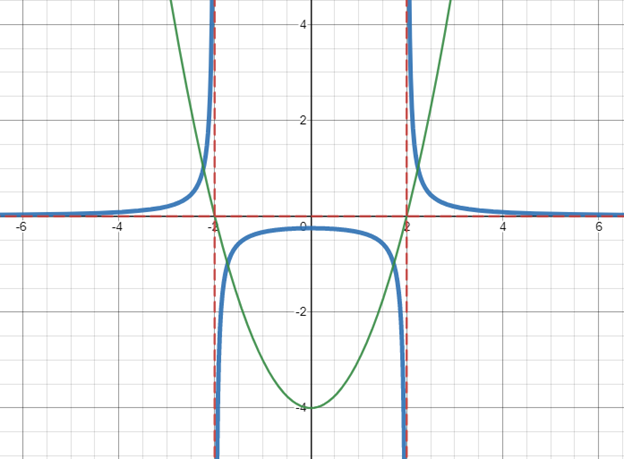
\includegraphics[scale = 0.5]{Images/PreCalcPictures/ReciprocalEx.png}}

\subsubsection{Inverse Functions}
The inverse of a function reverses the process represented by that function, interchanging $x$ and $y$ coordinates. The result is a reflection along the line $y=x$. Inverse notation is $f^{-1}(x)$ or $x=f(y)$.\\
Mapping notation: $(x,y)\rightarrow(y,x)$\\
To solve for the inverse of a function, switch $x$ and $y$ and then solve for $y$.\\
Ex: Inverse of $y=\frac{1}{2x+5}$
\begin{align*}
    x=&\frac{1}{2y+5}\\
    x(2y+5)=&1\\
    2y+5=&\frac{1}{x}\\
    2y=&\frac{1}{x}-5\\
    y=&\frac{1}{2x}-\frac{5}{2}
\end{align*}
Ex2: Inverse of $y=x^2+2x-2$
\begin{align*}
    x=&y^2+2y-2\\
    x=&y^2+2y+1-2+1\\
    x=&(y+1)^2-1\\
    x+1=&(y+1)^2\\
    \pm\sqrt{x+1}=&y+1\\
    y=&\pm\sqrt{y+1}-1
\end{align*}
\subsubsection{Square Root of a Function}
A square root function is the inverse of a quadratic. Because the inverse of a parabola does not meet the requirements of a function, we can restrict the range in order to make it a function. In doing this, we state that the square root must always be positive and this goes for all functions.
$$y=\sqrt{f(x)}$$
Mapping notation: $(x,y)\rightarrow(x,\sqrt{y})$\\
The square root of a function will travel in the same direction as the original function but the shape and value will be different.
For $f(x)<0$, $\sqrt{f(x)}$ is undefined\\
For $0<f(x)<1$, $\sqrt{f(x)}>f(x)$\\
For $f(x)>1$, $\sqrt{f(x)}<f(x)$\\
Note that we must restrict the domain of $x$ such that the value of $f(x)>0$\\
An interesting thing to note is that the square root of any downward opening parabola forms a semicircle.\\
\\
Solving radical equations:\\
Ex: $\sqrt{x-2}=4-x$
\begin{align*}
    &\text{Restrictions: }x-2\geq 0\Ra x\geq 2\\
    &\text{and }x-4\geq 0\Ra x\leq 4\\
    &(\sqrt{x-2})^2=(4-x)^2\\
    &x-2=16-8x+x^2\\
    &x^2-9x+18=0\\
    &(x-3)(x-6)=0\\
    &x=3,x=6\\
    &x=6\nleq 4\,\therefore \text{ not a solution}\\
    &\Ra x=3
\end{align*}
\subsubsection{Rational Functions}
Rational functions are an algebraic fraction with a numerator and denominator that are polynomials. In other words, it is a function divided by a function.\\
Ex: $\dfrac{x-7}{x^2-4x+3}$\\
\\
The graphs of rational functions can have a variety of features including asymptotes and holes. Asymptotes and holes occur at points where the function is not defined (divided by 0). These values for which the denominator is equal to 0 are called non-permissible value (NPVs).\\
Ex: NPVs of $\dfrac{x-7}{(x-3)(x-1)}$ are $x\neq3$ and $x\neq 1$\\
\\
Solving Rational Functions:\\
The x-intercepts of a rational function occur where the numerator is equal to 0 (given the denominator is not also 0).\\
Ex: $\dfrac{6-x}{2x}\Ra6-x=\Ra x=6$\\
\\
Simplifying Rational Expressions:\\
Some rational expressions can be factored and simplified.\\
Ex: $\dfrac{6-2x}{x^2-9}=\dfrac{-2(x-3)}{(x+3)(x-3)}$\\
The $(x-3)$ terms cancel, leaving $\dfrac{-2}{x+3}$.\\
Note that you must include all original NPVs. Otherwise, the simplified function would not be the same as the original. This new, simplified function will have a hole (removable discontinuity) at the point $x=3$, the term that was removed.\\
So, our final answer is $\dfrac{-2}{x+3}$ where $x\neq\pm3$\\
\\
Operations with Rational Expressions:\\
When dividing two rational expressions, we must take the NPVs of both expressions at the start and then once more after dividing.\\
Ex: $\dfrac{3x^2}{y^2}\div\dfrac{x}{y}\to$ NPVs: $y\neq0$\\
$\dfrac{3x^2y}{xy^2}\to$ NPVs: $y\neq0,\,x\neq0$\\
When adding and subtracting rational epressions, you must find the LCM and multiply the expressions accordingly as you do with regular addition and subtraction with fractions.\\
Ex: $\dfrac{5x}{x+2}+\dfrac{2x-3}{x-1}=\dfrac{5x(x-1)+(2x-3)(x+2)}{(x+2)(x-1)}$ where $x\neq-2,\,x\neq1$\\
\\
Asymptotes:\\
Vertical asymptotes occur at points where the function has NVPs that are not holes. For example, $\frac{1}{x}$ has a vertical asymptote at $x=0$. At these asymptotes, the function will curl up or down towards $y=\infty$ or $y=-\infty$.\\
Horizontal asymptotes are the end behavior of rational functions. As $x$ approaches positive or negative infinity, the function will either diverge (go to infinity) or approach a finite value as a horizontal asymptote.
\begin{itemize}
    \item If the degree of the numerator is greater than the degree of the denominator, $f(x)\to\pm\infty$
    \item If the degree of the numerator is the same as the degree of the denominator, $f(x)\to L$ where $L$ is some constant.
    \item If the degree of the numerator is less than the degree of the denominator, $f(x)\to 0$
\end{itemize}